\small

\section{Deviations and Audit}
\label{app:audit}

\subsection{Pre-specification audit}
Table~\ref{tab:audit} gives, for each spike, whether git shows the rule committed before the result. Timestamps are local commit times on one author clock; the repository has no external timestamping. ``YES'' means the rule text is in a commit strictly earlier than the first commit containing the result; ``UNPROVABLE'' means both arrive in one commit or the rule lived in a task prompt. No case was found in which git shows a rule committed after its result.

\begin{table}[htbp]
\centering
\caption{Git order of rule and result.}
\label{tab:audit}
\begin{tabular}{@{}p{3.3cm}p{9.2cm}l@{}}
\toprule
Spike & Rule and note & Order \\ \midrule
01, 02, 03a & Cards v1/v2, same snapshot commit as results; W1/W2 strengths set after a teacher-only look at TEST (spike02) & UNPROVABLE \\
03b, 05, 06, 07, 09b, 10b & Cards v2--v7.1 committed 1--4 h before results. Deviations: PPO recipe pre-lesson (03b); retroactive log entry (05); checkpoint selection added after round 1 (06); PPO not fixed before TEST (07); plant step changed after CAL tuning and dose curve run after locked TEST-B (10b) & YES \\
04 & H7 written in the result commit and amended after seeing the delay break the old C1 & UNPROVABLE, amended \\
11a, 13b & Rule in a task prompt or README of the result commit & UNPROVABLE \\
12a, 13a, 14a & Headline rule in the decision log earlier; details in the result commit. 13a: gate bias fell back to 6\,Nm and the gate was judged on $n{=}500$ instead of 200 & YES for headline \\
15a (TEST-C) & Cards v8 and v8.1 committed on their own about 2 h before the run; v8.1 re-trained L-dec4, predictions identical to the stored ones & YES \\
15b, 15c, 15d & Rules in README section 0 only; X1 (15b) and the 9-network extension (15c) added after results and labelled post hoc & UNPROVABLE \\
15e (TEST-D) & Card v9 committed on its own 1 h 22 min before the run; the code was uncommitted at run time, and the gated step was finished by the orchestrator with unchanged code & YES (card) \\
16a & Rule in README section 0, same commit as results; code uncommitted at run start & UNPROVABLE \\
learn\_demo & Not pre-specified; hyper-parameters chosen after one TEST look; stale, superseded by S3 re-run & NO \\
\bottomrule
\end{tabular}
\end{table}

\subsection{The v9 card is internally inconsistent for H16b}
The card's H16b rule is ``$B-\text{C-ens}$, 95\% CI upper end below +10\pp''. Its Holm step uses a one-sided bootstrap $p$ for $H_0$: difference $\ge 10$, which corresponds to the 90\% CI. On TEST-D the 95\% upper end is 10.6 (rule fails), the 90\% CI is [1.4, 9.8], and the one-sided $p$ is 0.0432, which would pass at $\alpha=0.05$ alone. We treat the rule text as binding, so H16b is not supported, and never write that the advantage is below 10\pp. The card's pre-written sentence for this outcome, applied on Holm-surviving verdicts, reads that the learned advantage may be $\ge10$\pp\ and that the paper rewrites K2 accordingly; Section~\ref{sec:k2} does so.

\subsection{Order of the classical upgrade (C-ens)}
The classical ensemble C-ens was built \emph{after} the learned ensemble B had beaten R0 on holdout (a first commit at 18:07 on the day of the study) and was frozen in a second commit at 20:31; its selection was written to a file before holdout and new-seed collection, and the v9 card was written at 20:32, after C-ens was frozen and before TEST-D. B$-$C-ens is therefore a pre-specified locked contrast, but the classical comparator was built with the learned result in view. The rule was developed first for the learned side and then given to the classical side. C-ens was chosen on CAL among 20 ensemble variants (B among 22) and uses the generative parameter distribution as a prior (a disclosed, non-neutral choice); no Laplace-width sensitivity run was made, and the multi-start classical family was degenerate (439 of 500 holdout episodes without a distinct second solution). On the pre-locked sets the contrast was B$-$C-ens +7.0\pp\ [2.6, 11.4] (holdout) and +4.0\pp\ [$-3.0$, 11.0] (new seeds), verdict UNCERTAIN by the README rule.

\subsection{Audit log scope}
The log has 111 lines: 47 from the demo-student script, 56 from one MJX evaluation, one each for juggling spikes 05, 06, 07 (05 and 06 retroactively), whip spike 09b, TEST-C and TEST-D, and two for spike 10b (TEST-B and TEST). The log is written only by the arena's \texttt{evaluate}. The TEST evaluations of spikes 01, 02, 03a, 03b and 04 ran outside it; spikes 15b--15d and 16a added no lines because guards block the locked sets. TEST (seeds 0--49) was reused across several spikes, on the same task for juggling (05, 06, 07).

\subsection{Equivalence summary (post hoc TOST)}
Equivalent within $\pm10$ (whole 90\% CI inside): S2 disturbed, S3 (all five students), S4 restitution (pilot), S5 oracle-PPO (legacy), S7 L-est-full, L-est-eff, PPO (13a) and OOD. Within $\pm5$ as well: S2 disturbed, S3 BC, MIP and flow, S5 oracle-PPO, S7 L-est-full and PPO. Not decidable: S1 (all four cells), S6 oracle-PPO (legacy), S8 best D-canon student. Learned clearly worse (90\% CI below $-10$): S2 clean, S4 mass and sensing (pilot), S5 PPO ($-23.8$) and SAC, S6 PPO ($-17.6$) and L-est, S8 D-multi students. Learned clearly better beyond $\pm10$: none.

\subsection{Full limitations}
\begin{enumerate}
\item \textbf{RL did not learn in the settings that matter most.} On realistic whip, 11 PPO and 2 SAC configurations tuned on CAL, three seeds of 3M steps and a 12M-step run all stayed within $-3$ to +2\pp\ of initialisation; in idealised whip all six PPO runs were flagged not learned; in juggling the residual stayed at 0.15--0.18\,Nm of a 12\,Nm cap and 4 of 6 runs chose the first checkpoint. The gate passed marginally, only after raising the exploration scale, among 8 gate runs. The S5 and S6 re-runs degrade the base by 23.8 and 17.6\pp, but each gate is a single-seed shot, the S5 gate is easy, the S6 budget is 3.2$\times$ classical, the recipe was not swept on the real condition, and the asymmetric-critic gate failed. The null is ``not learned under about 3--12M steps, one recipe per setting and about 13 tuned configurations on whip''.
\item \textbf{Holdout reuse.} HOLD was used to choose best-classical in spikes 09b and 10b (on 300 of the 500 seeds) and then as the main evaluation set in spikes 13a, 13b and 14a. R0 is 69.2\% on HOLD against 65.6, 65.6 and 66.4\% on TEST-B, TEST-C and TEST-D. The multimodal-teacher result, the group split, the fragility sweep and the 9-network extension have no locked-set confirmation.
\item \textbf{Realistic conditions are our own choice.} The friction value is an estimate.
\item \textbf{One simulator.} No second engine, no hardware.
\item \textbf{Concentration on whip.} Five of the eight settings are tracking or juggling, where headroom is small or absent.
\item \textbf{Unequal tuning knobs.} The classical side tuned 5--13 parameters with 750--9{,}050 episodes and received the generative distribution as bounds and priors; the learned side used $10^4$--$10^5$ episodes and simulator labels. In the estimator duel the classical side tried only three strengthened variants.
\item \textbf{Forking paths.} W1/W2 strengths set after seeing TEST (spike02); hyper-parameters chosen after one TEST look (learn\_demo); RL recipe repaired after round 1 (spike06); PPO not fixed before TEST (spike07); plant step changed after CAL tuning and dose curve after the locked TEST-B (spike10b); post hoc analyses in spikes 13b and 14a. There is no correction across spikes, so positive exceptions are exploratory.
\item \textbf{Pipeline noise.} Re-running identical estimator models with float-rounding changes moved holdout success by up to 3.6\pp\ per model, comparable to several reported differences.
\item \textbf{Power and equivalence.} Most pre-specified tests had CI half-widths of 4--9\pp\ (TEST $n{=}50$ comparisons up to about 15\pp). ``No side wins at the 10\pp\ bar'' is not an equivalence test. Differences of +1 to +5\pp\ (for example the three-model ensemble, +4.8\pp\ [$-0.8$, 10.4]) cannot be excluded.
\item \textbf{Fairness of the plan-selection duel.} See the C-ens paragraph above; the learned side used 13{,}120 training episodes with simulator labels, and both sides are frozen by the v9 card.
\item \textbf{Pre-specified versus post hoc.} Besides the earlier spikes marked YES in Table~\ref{tab:audit}, only cards v8, v8.1 and v9 were committed on their own before their runs; spike15b/15c/15d rules are README-only; the 9-network extension, B9, the reverse-order ladder, S6-X1 and L-ens/C-MAP are post hoc or descriptive.
\item \textbf{Numerical warnings.} The check of the 125{,}555 warnings (4{,}621 on holdout) was a re-run on 100 holdout episodes; the full holdout and TEST-D check was not repeated. No executed episode record contained a non-finite outcome.
\item \textbf{Order of the classical upgrade.} See above.
\end{enumerate}

\section{Budgets and the RL Gate}
\label{app:budget}

\begin{table}[htbp]
\centering
\caption{Budget by spike (episodes, steps, wall-clock where reported). Counting conventions differ between steps, episodes and probe-equivalents; the spike09b classical design cost (about 1{,}300 episodes) is an estimate.}
\label{tab:budget}
\begin{tabular}{@{}p{2.2cm}p{7.3cm}p{3.7cm}@{}}
\toprule
Spike & Classical side / learned side & Ratio \\ \midrule
03a (tracking) & classical tuning 6.4M--9.0M steps; RL 2M steps per policy & classical about 7.7$\times$ (C1+C2, one weakness) \\
06 (juggling) & classical 118.2M steps; RL 121.0M & 1.02$\times$ \\
07 (juggling) & PPO and oracle about 144M steps (107.6M without out-of-memory reruns); SAC 27M & 2.3$\times$ (1.7$\times$) \\
10b (whip) & classical 11{,}300 episodes (2$\times$ cap 22{,}600); learned methods each inside the cap & within cap \\
13a (whip RL) & about 160k episodes vs 22.6k classical & about 7$\times$ \\
14a (estimator duel) & learned about 13{,}120 episode-equivalents vs classical about 1{,}500 & 9--17$\times$ \\
15b (S6 re-run) & 33k episodes vs 10{,}350 classical & 3.2$\times$ \\
16a (catch / toss / Push-T) & classical tuning 16{,}200 / 10{,}200 / 2{,}100 episodes; PPO 16{,}227 / 10{,}222 / 2{,}114 & about 1$\times$ \\
\bottomrule
\end{tabular}
\end{table}

\begin{table}[htbp]
\centering
\caption{All RL gates and checkpoint decisions (single seed or best-of-$N$ flagged). Differences are paired learned minus initialisation (gates) or minus base (real conditions), in pp.}
\label{tab:gates}
\begin{tabular}{@{}p{4.4cm}p{5.3cm}p{3.5cm}@{}}
\toprule
Gate or run & What is single-seed or best-of & Result \\ \midrule
13a gate, log-std $-3.5$ (default) & gate set $n{=}200$ & $-3.0$ [$-8.5$, +2.5] \\
13a gate, log-std $-2.0$ & HOLD $n{=}500$ & +7.8 [3.0, 12.8] \\
13a gate, log-std $-1.5$, 3M steps & best of 8 runs, CAL-selected & +10.2 [4.8, 15.6] \\
13a gate, SAC & single seed & +1.8 [$-3.4$, 7.0] \\
13a real condition & 11 PPO + 2 SAC configs, one seed each; confirmation 3 seeds & HOLD $-2.1$ [$-5.2$, 1.1]; NEW $-1.3$ [$-6.5$, 3.8]; 12M steps $-0.6$ [$-4.6$, 3.4] \\
15b S6 gate (bias 6\,Nm) & one seed, one shot & +15.4 [10.2, 20.6] \\
15b S5 gate (bias 1\,Nm) & one seed, one shot; easy gate & +63.2 [58.8, 67.4] \\
15b S6-X1 (weak base, post hoc) & CAL picks looked like +5.0, +11.5, +5.0 and vanished on disjoint seeds & holdout $-5.0$ [$-8.7$, $-1.5$]; fresh $-3.3$ [$-8.7$, +2.0] \\
15c asymmetric critic & two seeds, one extra attempt allowed; failed & +7.2 [2.0, 12.4]; +1.2 [$-4.0$, 6.4] \\
\bottomrule
\end{tabular}
\end{table}

\section{Replication on Reused and Fresh Seeds, and Sensitivity}
\label{app:replication}

\begin{table}[htbp]
\centering
\caption{Headroom ladder on HOLD ($n{=}500$) and NEW ($n{=}200$): success \% [95\% CI].}
\label{tab:replication}
\begin{tabular}{@{}lll@{}}
\toprule
Rung & HOLD & NEW \\ \midrule
R0 fitted & 69.2 [65.2, 73.2] & 69.0 [62.5, 75.5] \\
R1 true $\theta$ & 86.0 [83.0, 89.0] & 82.0 [76.5, 87.0] \\
R2 + chain state & 89.0 [86.2, 91.6] & 89.5 [85.0, 93.5] \\
R3 oracle at rest, waits 0.6\,s & 88.2 [85.4, 91.0] & 85.5 [80.5, 90.5] \\
R4 oracle & 90.8 [88.2, 93.2] & 87.5 [82.5, 92.0] \\
R5 canonical oracle & 92.0 [89.6, 94.2] & 92.5 [88.5, 96.0] \\
L-est-full (3 nets) & 64.7 [62.1, 67.3] & 66.7 [62.5, 70.8] \\
R1$-$R0 & +16.8 [12.0, 21.6] & +13.0 [4.5, 21.5] \\
R2$-$R1 & +3.0 [$-1.0$, 7.0] & +7.5 [1.0, 14.0] \\
R4$-$R2 & +1.8 [$-1.6$, 5.4] & $-2.0$ [$-8.0$, 4.0] \\
\bottomrule
\end{tabular}
\end{table}

On TEST-B the total headroom (T-oracle minus the best classical) is +23.6\pp\ [18.8, 28.4]. The R2$-$R1 step is significant on NEW but not on HOLD, and the R4$-$R2 sign flips, so these blocks are not replicated as real; the earlier suggestion that the oracle gap was mostly probe time and chain state was a winner's-curse artefact and is superseded. A post hoc group split on HOLD (wrong damping 18.4\pp, per-link masses 16.2, length 7.4, friction 4.6 when only that group is wrong) is non-additive and not used for claims.

\begin{table}[htbp]
\centering
\caption{Actuator-noise sweep, HOLD seeds 1100--1299 ($n{=}200$), paired drop relative to the $\times$1 noise level (pp [95\% CI]). Methods frozen, not re-tuned per level.}
\label{tab:fragility}
\begin{tabular}{@{}lrrr@{}}
\toprule
Method & $\times$2 & $\times$4 & $\times$8 \\ \midrule
T-adapt3-full & +0.5 [$-7.5$, 8.5] & $-12.5$ [$-21.5$, $-3.5$] & $-14.5$ [$-24.0$, $-5.0$] \\
L-est-full & +7.0 [$-1.5$, 15.5] & +4.0 [$-5.0$, 13.0] & $-0.5$ [$-10.0$, 9.0] \\
T-oracle & +0.5 [$-3.0$, 4.0] & $-3.5$ [$-7.0$, 0.0] & $-1.0$ [$-4.0$, 1.5] \\
\bottomrule
\end{tabular}
\end{table}

Under sensor noise the ordering is not distinguishable (T-adapt3-full $-10.0$\pp\ [$-19.5$, $-1.0$] at $\times$2, L-est-full +0.5 [$-8.5$, 9.5]). The paired difference of the two drops at actuator noise $\times$4 is $-16.5$\pp\ [$-28.5$, $-5.0$].

\textbf{Dose curve and out-of-distribution.} On HOLD ($n{=}200$ per level; run after the locked TEST-B), success of best classical / L-est-full / L-est-eff / T-oracle is 71.0 / 64.3 / 67.5 / 92.0 at $\times$0.5, 69.5 / 61.2 / 61.2 / 89.5 at $\times$1 and 53.0 / 60.3 / 56.8 / 91.0 at $\times$2. The paired L-est-full minus classical is $-6.7$ [$-13.5$, 0.2], $-8.3$ [$-16.2$, $-0.3$] and +7.3 [$-0.0$, 14.7]: a single point at the strongest condition. For estimators trained or tuned at $\times$0.5 and $\times$2 and evaluated at $\times$1, L-est-OOD minus T-adapt3-OOD is +5.9\pp\ [1.1, 10.8] on TEST-B, but the classical OOD variant was tuned with fewer episodes (350). Classical was not re-tuned at $\times$2.

\textbf{Estimator duel on reused sets.} L-dec4$-$R0 is +1.1\pp\ [$-3.3$, 5.7] on HOLD and +0.5\pp\ [$-6.7$, 7.8] on NEW (recovered 0.07 and 0.04). The post hoc three-model ensemble gives +4.8\pp\ [$-0.8$, 10.4] and +3.5\pp\ [$-5.0$, 12.0]. Adding independent Gaussian noise of the learned estimator's size to the true parameters gives 65.0\% (noise $\times$1) and 74.0\% ($\times$0.5) against 86.0\% for the true parameters, a post hoc diagnostic that the planner needs errors well below the learned error. Classical strengthening (MAP prior, multi-start, K-step resets) did not improve the pipeline.

\section{Multimodal Teacher (K4) and Privileged Distillation}
\label{app:k4}

\begin{figure}[htbp]
\centering
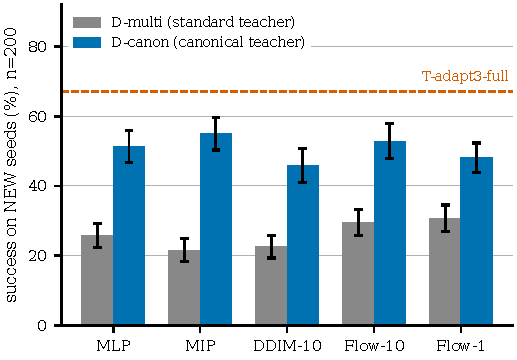
\includegraphics[width=0.5\textwidth]{fig_k4}
\caption{Five students trained on data from the standard multimodal teacher (D-multi) or the canonical teacher (D-canon), NEW seeds ($n{=}200$), mean over three training seeds, 95\% CI. The dashed line is T-adapt3-full on the same seeds.}
\label{fig:k4}
\end{figure}

Canonicalising the teacher raised each student by: MLP 25.7\pp\ [19.8, 31.5], MIP 33.5\pp\ [28.0, 38.8], DDIM-10 23.3\pp\ [17.7, 29.0], flow-10 23.3\pp\ [17.3, 29.2], flow-1 17.5\pp\ [11.7, 23.5]. On D-multi, the differences from the MLP are flow-1 +5.0 [$-0.3$, 10.2], flow-10 +3.8 [$-1.0$, 8.7], diffusion $-3.2$ [$-7.7$, 1.3] and MIP $-4.2$ [$-8.8$, 0.5]. The canonical oracle teacher reaches 96.0\% [93.0, 98.5] and T-adapt3-full 67.0\% [60.5, 73.5], so the best D-canon student (MIP, 55.0\%) is $-12.0$\pp\ [$-19.8$, $-4.0$] below it (best student chosen on the same final episodes, which is optimistic for the learned side); all D-multi students are 36.3--45.5\pp\ below. In the earlier privileged-teacher study (NEW $n{=}200$), the canonical oracle reached 92.5\%, T-adapt3-full 60.0\% and the students 58.0--59.5\%. Seed-to-seed spread was 5--15\pp. The data are NEW only, behaviour cloning only (no DAgger) and one data scale (400 scenarios).

\section{Breadth: Other Tasks and Classical Pilots}
\label{app:breadth}

\textbf{Residual PPO on catch, toss and Push-T.} Table~\ref{tab:16a} gives the mini-comparisons (rules in a spike README, order not provable from git; breadth only). Catch and Push-T ties are at the ceiling, where a +10\pp\ win is arithmetically impossible, and toss is uninterpretable because its gate failed four times (best +1.3\pp). Local and remote runs of 30 episodes had identical outcomes, lengths and joint trajectories; the only difference was 7.8e-16 in a Push-T summary statistic.

\begin{table}[htbp]
\centering
\caption{Residual PPO on the CAL-tuned strongest classical, learned minus classical (pp [95\% CI]).}
\label{tab:16a}
\begin{tabular}{@{}lllllll@{}}
\toprule
Task & Gate (pp) & Classical HOLD / NEW & HOLD ($n{=}500$) & NEW ($n{=}200$) & Verdict \\ \midrule
Catch & +54.0 [48.3, 59.7] & 0.992 / 1.000 & $-0.5$ [$-1.1$, 0.1] & $-0.7$ [$-1.8$, 0.0] & tie (ceiling) \\
Push-T & +61.3 (1 seed) & 0.990 / 0.995 & +0.4 [$-0.4$, 1.2] & $-1.5$ [$-3.5$, 0.0] & tie (ceiling) \\
Toss & failed 4 times & 0.680 / 0.685 & +0.6 [$-1.2$, 2.4] & $-1.0$ [$-3.0$, 1.0] & no verdict \\
\bottomrule
\end{tabular}
\end{table}

\textbf{Classical pilots (demo seeds, no learned comparison).} On the tracking ladder ($n{=}5$) the RMSE is 0.0074 (PID), 0.0061 (CTC+LQR), 0.0056 (iLQR), 0.0056 (iLQR-MPC) and 0.0073 (MPPI) rad. Catching succeeds 19 of 20 without error but 6 of 20 with 10\,ms ball-position delay; whip with a chain 10\% shorter succeeds 12 of 20; Push-T succeeds 19 of 20 with 20\,ms sensor delay and 0 of 20 with 30\,ms. These pilots motivated choosing whip and are not paper claims. An MJX-trained PPO reproduced the CPU PPO within CI with 4.7e6 steps/s on 4096 environments; this engineering result is not used for K1--K4.
